\chapter{Architettura e Design del Sistema}
\label{cha:architettura_e_design_del_sistema}
In questo capitolo vengono illustrate in dettaglio le scelte architetturali, le tecnologie adottate e i principi di design che guidano lo sviluppo del sistema DietiEstates. L'obiettivo è fornire una visione chiara della struttura software, giustificando le decisioni prese in ottica di manutenibilità, scalabilità e robustezza, secondo le migliori pratiche dell'ingegneria del software.

\section{Architettura del Sistema}
\label{sec:architettura_del_sistema}
Il sistema è stato progettato seguendo un'architettura multi-tier, specificamente un'architettura a tre livelli (Three-Tier Architecture), che separa nettamente la logica di presentazione, la logica di business e la gestione dei dati. Questo approccio favorisce la modularità, il disaccoppiamento tra i componenti e la possibilità di sviluppare, manutenere e scalare i singoli livelli in modo indipendente.

\subsection{Livello di Presentazione (Presentation Tier)}
Il livello di presentazione è costituito da un'applicazione web di tipo Single-Page Application (SPA), sviluppata con il framework Angular. Questa applicazione viene eseguita interamente nel browser dell'utente e ha la responsabilità di renderizzare l'interfaccia grafica, gestire le interazioni dell'utente e comunicare con il livello di business tramite chiamate API. La scelta di una SPA permette di offrire un'esperienza utente fluida e reattiva, simile a quella di un'applicazione desktop, minimizzando i tempi di attesa grazie al caricamento asincrono dei dati.

\subsection{Livello di Business (Application Tier)}
Il cuore del sistema risiede nel livello di business, un'applicazione backend sviluppata in Java utilizzando il framework Spring Boot. Questo livello espone un'interfaccia RESTful API sicura, attraverso la quale il client (l'applicazione Angular) può accedere alle funzionalità del sistema. Le responsabilità di questo tier includono:
\begin{itemize}
    \item \textbf{Gestione della Logica di Business:} Implementazione di tutte le logiche applicative, come la gestione degli annunci immobiliari, la gestione degli utenti e dei loro ruoli.
    \item \textbf{Autenticazione e Autorizzazione:} messa in sicurezza degli endpoint dell'API tramite Spring Security, gestendo l'autenticazione degli utenti (login) e l'autorizzazione basata sui ruoli (utente, agente, amministratore).
    \item \textbf{Comunicazione con il Livello Dati:} Interazione con il database PostgreSQL per il salvataggio e il recupero persistente delle informazioni.
\end{itemize}
La comunicazione tra il Presentation Tier e l'Application Tier avviene tramite il protocollo HTTP/S, con scambio di dati in formato JSON (JavaScript Object Notation), uno standard leggero e facilmente interpretabile da entrambi i sistemi.

\subsection{Livello Dati (Data Tier)}
Il livello dati è responsabile della persistenza delle informazioni. È costituito da un database relazionale (ad esempio PostgreSQL) che memorizza tutti i dati dell'applicazione, come le anagrafiche degli utenti, i dettagli degli immobili e le agenzie immobiliari con i loro agenti.

L'accesso a questo livello è gestito esclusivamente dall'Application Tier, che si avvale di un Object-Relational Mapper (ORM) come Hibernate, tramite l'astrazione offerta da Spring Data JPA. L'uso di un ORM astrae la complessità del linguaggio SQL, permettendo agli sviluppatori di interagire con il database attraverso oggetti Java (Entity), migliorando la manutenibilità e la portabilità del codice.

\section{Tecnologie Adottate}
\label{sec:tecnologie_adottate}
La selezione delle tecnologie è stata guidata da criteri di maturità, supporto della comunità, produttività e aderenza agli standard di mercato.

\subsection{Backend}
\begin{itemize}
    \item \textbf{Java:} Linguaggio di programmazione robusto, orientato agli oggetti e indipendente dalla piattaforma, ampiamente utilizzato per lo sviluppo di applicazioni enterprise complesse e performanti.
    \item \textbf{Spring Boot:} Framework che semplifica drasticamente lo sviluppo di applicazioni basate su Spring. È stato scelto per la sua capacità di auto-configurazione, la gestione integrata delle dipendenze e l'ecosistema completo che include moduli per la sicurezza (Spring Security), l'accesso ai dati (Spring Data JPA) e la creazione di API REST (Spring Web).
    \item \textbf{JPA/Hibernate:} Standard per la persistenza dei dati in Java. Hibernate, come implementazione JPA, gestisce la mappatura degli oggetti Java alle tabelle del database, semplificando le operazioni CRUD e le query complesse.
    \item \textbf{Maven:} Strumento di build automation e gestione delle dipendenze, utilizzato per definire la struttura del progetto, compilare il codice sorgente e gestire le librerie di terze parti.
    \item \textbf{Docker:} Piattaforma di containerizzazione utilizzata tramite Docker Compose per definire e orchestrare l'ambiente di sviluppo e produzione, garantendo coerenza e replicabilità tra le diverse macchine e semplificando il deployment.
\end{itemize}

\subsection{Approfondimento: Sicurezza con Spring Security e OpenID Connect}

Oltre alle scelte architetturali di alto livello, sono stati adottati specifici pattern di progettazione e configurazioni di sicurezza avanzate per garantire la robustezza, la manutenibilità e la sicurezza del sistema.

Per garantire un elevato livello di sicurezza nell'accesso alle risorse del sistema, è stato adottato Spring Security in combinazione con il protocollo OpenID Connect (OIDC). Questa scelta consente di implementare un sistema di autenticazione e autorizzazione robusto e scalabile, sfruttando le funzionalità offerte da provider di identità esterni.

Spring Security fornisce un framework completo per la gestione della sicurezza delle applicazioni Java, offrendo funzionalità come l'autenticazione degli utenti, l'autorizzazione basata sui ruoli e la protezione contro le vulnerabilità comuni (es. CSRF, XSS). Integrando OIDC, il sistema può delegare l'autenticazione a un Identity Provider (IdP) esterno, che gestisce in modo sicuro le credenziali degli utenti e fornisce token di accesso standardizzati. Questo approccio presenta diversi vantaggi:
\begin{itemize}
    \item \textbf{Sicurezza Migliorata:} La gestione delle credenziali è affidata a un provider specializzato, riducendo il rischio di vulnerabilità legate alla gestione interna delle password.
    \item \textbf{Scalabilità:} L'utilizzo di un IdP esterno consente di scalare facilmente il sistema di autenticazione senza dover implementare soluzioni personalizzate.
    \item \textbf{Esperienza Utente Unificata:} Gli utenti possono utilizzare le stesse credenziali per accedere a più applicazioni, migliorando l'usabilità e riducendo la necessità di gestire più account.
\end{itemize}
L'implementazione di Spring Security con OIDC prevede la configurazione del client OIDC all'interno dell'applicazione Spring Boot, la definizione delle regole di accesso alle risorse protette e la gestione dei token di accesso per autorizzare le richieste API.

\paragraph{Il design pattern Factory per la gestione dei vari providers}
\label{ssec:factory_pattern_oauth2}
Per gestire l'autenticazione tramite provider esterni (es. Google) secondo i protocolli OAuth2 e OpenID Connect, è stato implementato il \textbf{Factory Pattern}. Questa scelta di design è cruciale per disaccoppiare la logica di gestione dell'autenticazione dalle implementazioni specifiche di ciascun provider.

Il cuore di questo pattern è rappresentato dall'interfaccia \texttt{OAuth2UserInfo}, che definisce un contratto comune per l'estrazione degli attributi di un utente (come ID, nome, email) a prescindere dal provider. Per ogni provider supportato, viene creata una classe concreta (es. \texttt{GoogleOAuth2UserInfo}) che implementa questa interfaccia, sapendo come mappare la struttura dati, spesso eterogenea, restituita da quel provider.

La classe \texttt{OAuth2UserInfoFactory} agisce come "fabbrica": il suo metodo principale riceve in input il nome del provider e la mappa di attributi dell'utente, e restituisce l'istanza della classe concreta appropriata. In questo modo, i servizi che gestiscono il processo di login (\texttt{CustomOAuth2UserService} e \texttt{CustomOidcUserService}) non devono contenere logica condizionale (if/else o switch) per i diversi provider. Essi interagiscono esclusivamente con l'astrazione \texttt{OAuth2UserInfo}, favorendo il riutilizzo del codice e rendendo il sistema facilmente estensibile: per supportare un nuovo provider, è sufficiente creare una nuova implementazione dell'interfaccia e aggiornare la factory, senza modificare i servizi esistenti.

\paragraph{Gestione della sicurezza con la Security Filter Chain}
\label{ssec:security_filter_chain}
La sicurezza dell'applicazione backend è gestita da Spring Security attraverso una catena di filtri (\textbf{Security Filter Chain}). Questo approccio, che implementa il pattern Chain of Responsibility, permette di applicare una serie di controlli di sicurezza a ogni richiesta HTTP in arrivo.

La configurazione, definita nella classe \texttt{SecurityFilterConfig}, stabilisce l'ordine e il comportamento di questi filtri. Le principali responsabilità configurate includono:
\begin{itemize}
    \item \textbf{Autorizzazione degli Endpoint:} Viene definita una politica di accesso granulare per i diversi percorsi dell'API. Ad esempio, gli endpoint relativi all'autenticazione (es. \texttt{/api/auth/**}) sono resi pubblici, mentre altre aree richiedono ruoli specifici (es. \texttt{/api/admin/**} richiede il ruolo di \texttt{ADMIN}).
    \item \textbf{Gestione delle Sessioni:} L'applicazione è configurata per essere \textit{stateless}, ovvero non viene creata alcuna sessione utente sul server. Questa è una scelta fondamentale per le API RESTful, in quanto garantisce la scalabilità e semplifica il bilanciamento del carico. L'autenticazione di ogni richiesta è affidata a un token.
    \item \textbf{Integrazione OIDC e OAuth2:} La catena è configurata per intercettare e gestire i flussi di login con provider esterni, delegando il processo ai servizi specifici come \texttt{CustomOidcUserService}.
    \item \textbf{Filtri Personalizzati:} È stato inserito un filtro custom, \texttt{AuthFilter}, posizionato strategicamente all'interno della catena. Questo filtro ha il compito di ispezionare l'header \texttt{Authorization} di ogni richiesta, estrarre e validare il JSON Web Token (JWT) e, in caso di successo, popolare il \texttt{SecurityContext} di Spring. Questo passaggio è ciò che permette al resto dell'applicazione di identificare l'utente autenticato e i suoi ruoli per le successive richieste API.
\end{itemize}

\paragraph{Access token JWT e Refresh Tokens}
Per garantire un'autenticazione sicura e scalabile, il sistema utilizza JSON Web Tokens (JWT) come access token per autorizzare le richieste API. I JWT sono token compatti e auto-contenuti che trasportano informazioni sull'utente e sui suoi privilegi in modo sicuro. Quando un utente effettua il login tramite OIDC, riceve un access token JWT che deve essere incluso nelle intestazioni delle richieste API per accedere alle risorse protette. Questo approccio consente di evitare la necessità di mantenere sessioni lato server, migliorando la scalabilità dell'applicazione.

Accanto agli access token, il sistema implementa anche l'uso di refresh token. I refresh token sono token a lunga durata che consentono agli utenti di ottenere nuovi access token senza dover effettuare nuovamente il login. Quando un access token scade, l'applicazione può utilizzare il refresh token per richiedere un nuovo access token all'IdP, migliorando l'esperienza utente e mantenendo la sicurezza delle sessioni.

\begin{center}
    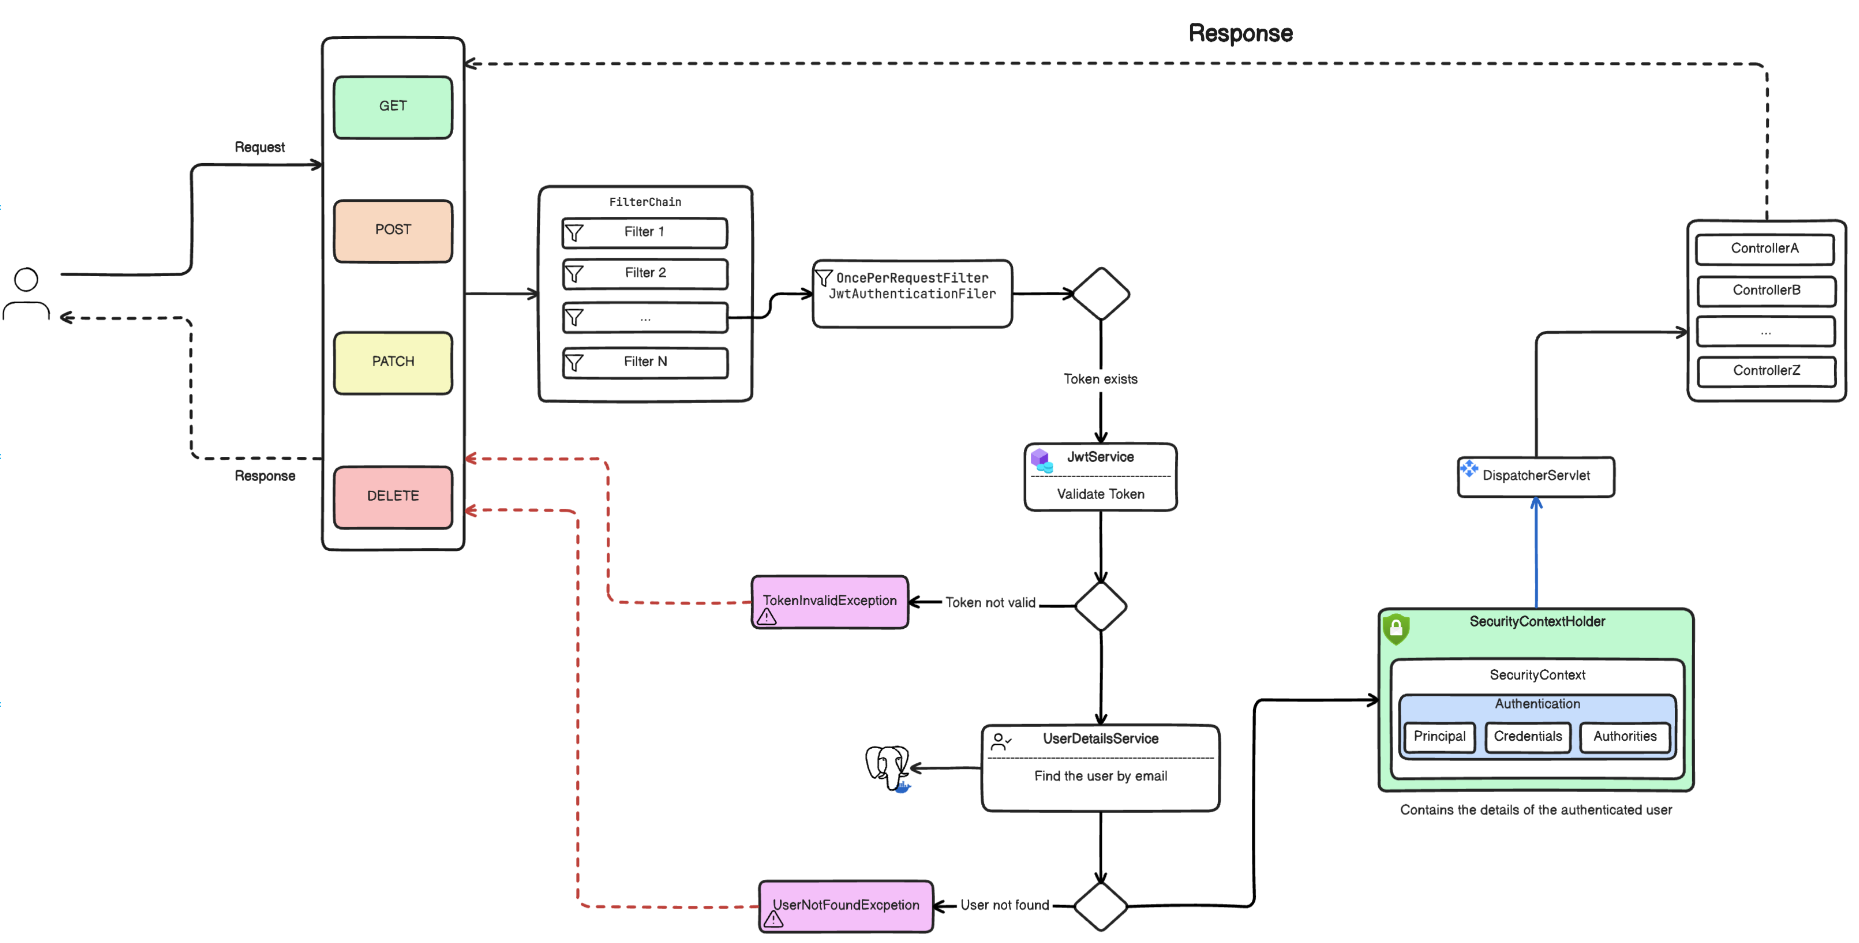
\includegraphics[width=0.75\textwidth]{res/security.png}
\end{center}

\subsection{Frontend}
\begin{itemize}
    \item \textbf{Angular:} Framework client-side basato su TypeScript, sviluppato da Google. È stato scelto per la sua architettura a componenti, che promuove la riusabilità del codice, e per il suo potente sistema di dependency injection, che facilita la scrittura di codice modulare e testabile.
    \item \textbf{TypeScript:} Superset di JavaScript che introduce la tipizzazione statica. Il suo utilizzo migliora la robustezza del codice, previene errori comuni in fase di sviluppo e aumenta la manutenibilità a lungo termine del progetto.
    \item \textbf{OpenAPI Generator:} Strumento fondamentale per l'integrazione tra frontend e backend. A partire dalla specifica OpenAPI (precedentemente nota come Swagger) esposta dal backend, questo strumento genera automaticamente un client API TypeScript completo e type-safe. Questo approccio riduce drasticamente il rischio di disallineamenti e è un pilastro per lo sviluppo contract-first.
    \item \textbf{HTML5 e CSS3:} Standard web utilizzati per la strutturazione semantica delle pagine e per la loro stilizzazione, garantendo compatibilità con i browser moderni e la possibilità di implementare design responsive.
\end{itemize}

\section{Design dell'Interfaccia Utente (UI)}
\label{sec:design_dell_interfaccia_utente_ui}
Il design dell'interfaccia utente è stato concepito per essere pulito, intuitivo e funzionale, con l'obiettivo di massimizzare l'usabilità per le diverse categorie di utenti (visitatori, clienti, agenti e amministratori).

\begin{itemize}
    \item \textbf{Approccio User-Centric:} Ogni elemento dell'interfaccia è stato pensato mettendo al centro le esigenze dell'utente. La navigazione è stata strutturata in modo logico e coerente, permettendo un facile accesso alle funzionalità principali come la ricerca di immobili, la gestione del proprio profilo e, per gli utenti privilegiati, la gestione degli annunci e degli agenti.
    \item \textbf{Coerenza Visiva e Riusabilità:} L'adozione di un'architettura a componenti, nativa in Angular, ha permesso di creare elementi riutilizzabili (es. le card degli annunci, i campi dei form, la navbar). Questo non solo accelera lo sviluppo, ma garantisce anche una forte coerenza visiva e comportamentale in tutta l'applicazione, rendendo l'esperienza utente più prevedibile e confortevole.
    \item \textbf{Responsive Design:} L'interfaccia è stata progettata con un approccio "mobile-first", garantendo che l'applicazione sia perfettamente fruibile su un'ampia gamma di dispositivi, dai desktop agli smartphone. L'utilizzo di tecniche CSS moderne come Flexbox e Grid consente al layout di adattarsi fluidamente alle diverse dimensioni dello schermo.
    \item \textbf{Feedback all'Utente:} Il sistema fornisce un feedback visivo costante per ogni azione intrapresa dall'utente. Indicatori di caricamento (spinner) durante le chiamate asincrone, messaggi di successo o di errore chiari e validazione contestuale dei form sono tutti elementi implementati per migliorare la comunicazione tra il sistema e l'utente, riducendo l'incertezza e migliorando la percezione di reattività dell'applicazione.
\end{itemize}
L'ispirazione per il layout e l'esperienza utente è tratta dai principali portali immobiliari moderni, cercando di adottare convenzioni già familiari agli utenti per ridurre la curva di apprendimento.
